% This file was created by matlab2tikz.
%
%The latest updates can be retrieved from
%  http://www.mathworks.com/matlabcentral/fileexchange/22022-matlab2tikz-matlab2tikz
%where you can also make suggestions and rate matlab2tikz.
%
\definecolor{mycolor1}{rgb}{0.85000,0.95000,1.00000}%
\definecolor{mycolor2}{rgb}{0.95000,0.85000,0.85000}%
\definecolor{mycolor3}{rgb}{0.06600,0.44300,0.74500}%
\definecolor{mycolor4}{rgb}{0.12941,0.12941,0.12941}%
%
\begin{tikzpicture}

\begin{axis}[%
width=0.951\textwidth,
height=0.058\textheight,
at={(0\textwidth,0.162\textheight)},
scale only axis,
xmin=0,
xmax=59,
ymin=0,
ymax=401.1,
ylabel style={font=\color{mycolor4}},
ylabel={Packets/s},
axis background/.style={fill=white},
title style={font=\bfseries\color{mycolor4}},
title={toolbox-0 — sub-managed-1},
axis x line*=bottom,
axis y line*=left,
xmajorgrids,
ymajorgrids,
grid=both,
tick align=outside,
scaled y ticks=true,
title style={yshift=1.0ex}
]

\addplot[area legend, draw=none, fill=mycolor1, fill opacity=0.35, forget plot]
table[row sep=crcr] {%
x	y\\
13	0\\
23	0\\
23	401.1\\
13	401.1\\
}--cycle;

\addplot[area legend, draw=none, fill=mycolor2, fill opacity=0.25, forget plot]
table[row sep=crcr] {%
x	y\\
38	0\\
43	0\\
43	401.1\\
38	401.1\\
}--cycle;
\addplot [color=mycolor3, forget plot]
  table[row sep=crcr]{%
0	0\\
12	0\\
13	4\\
14	10\\
22	10\\
23	6\\
24	0\\
37	0\\
38	10\\
39	40\\
41	40\\
42	382\\
43	4\\
45	0\\
46	0\\
47	2\\
48	0\\
49	2\\
50	0\\
51	2\\
52	0\\
53	2\\
54	2\\
55	0\\
56	0\\
57	4\\
58	0\\
59	0\\
};
\end{axis}

\begin{axis}[%
width=0.951\textwidth,
height=0.058\textheight,
at={(0\textwidth,0.081\textheight)},
scale only axis,
xmin=0,
xmax=59,
ymin=0,
ymax=10.5,
ylabel style={font=\color{mycolor4}},
ylabel={Packets/s},
axis background/.style={fill=white},
title style={font=\bfseries\color{mycolor4}},
title={toolbox-0 — sub-managed-2},
axis x line*=bottom,
axis y line*=left,
xmajorgrids,
ymajorgrids,
grid=both,
tick align=outside,
scaled y ticks=true,
title style={yshift=1.0ex}
]

\addplot[area legend, draw=none, fill=mycolor1, fill opacity=0.35, forget plot]
table[row sep=crcr] {%
x	y\\
13	0\\
23	0\\
23	10.5\\
13	10.5\\
}--cycle;

\addplot[area legend, draw=none, fill=mycolor2, fill opacity=0.25, forget plot]
table[row sep=crcr] {%
x	y\\
38	0\\
43	0\\
43	10.5\\
38	10.5\\
}--cycle;
\addplot [color=mycolor3, forget plot]
  table[row sep=crcr]{%
0	0\\
12	0\\
13	4\\
14	10\\
22	10\\
23	6\\
24	0\\
31	0\\
32	1\\
33	0\\
41	0\\
42	2\\
43	0\\
46	0\\
47	2\\
48	0\\
59	0\\
};
\end{axis}

\begin{axis}[%
width=0.951\textwidth,
height=0.058\textheight,
at={(0\textwidth,0\textheight)},
scale only axis,
xmin=0,
xmax=59,
xlabel style={font=\color{mycolor4}},
xlabel={Time (s)},
ymin=0,
ymax=2.1,
ylabel style={font=\color{mycolor4}},
ylabel={Packets/s},
axis background/.style={fill=white},
title style={font=\bfseries\color{mycolor4}},
title={toolbox-1 — sub-managed-2},
axis x line*=bottom,
axis y line*=left,
xmajorgrids,
ymajorgrids,
grid=both,
tick align=outside,
scaled y ticks=true,
title style={yshift=1.0ex}
]

\addplot[area legend, draw=none, fill=mycolor1, fill opacity=0.35, forget plot]
table[row sep=crcr] {%
x	y\\
13	0\\
23	0\\
23	2.1\\
13	2.1\\
}--cycle;

\addplot[area legend, draw=none, fill=mycolor2, fill opacity=0.25, forget plot]
table[row sep=crcr] {%
x	y\\
38	0\\
43	0\\
43	2.1\\
38	2.1\\
}--cycle;
\addplot [color=mycolor3, forget plot]
  table[row sep=crcr]{%
0	0\\
7	0\\
8	2\\
9	0\\
41	0\\
42	2\\
43	0\\
59	0\\
};
\end{axis}
\end{tikzpicture}%